Figure~\ref{fig:cmp_res} shows the results obtained by the proposed AKDE compared to SPADES~\cite{bunea2010spades} method. We set $N=500, \gamma = 7, pq = 1500$ for this experiment.
\begin{figure}[hbt!]
\vspace{-2cm}
    \hspace{-2cm}
    \begin{tabular}{ccc}
    $f_0$& $f_1$ & $f_2$\\
         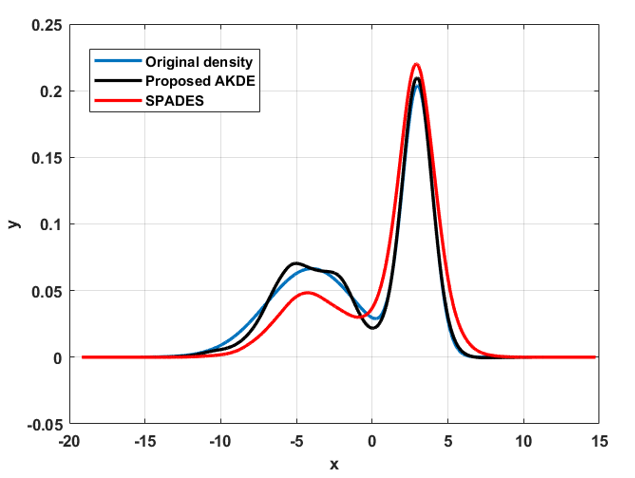
\includegraphics[scale = 0.42]{Figures/Adaptive/cmp_reults/0.PNG}&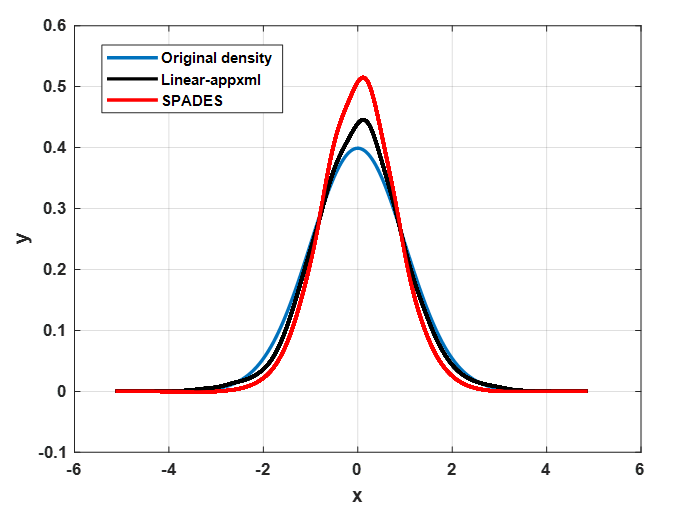
\includegraphics[scale = 0.38]{Figures/Adaptive/cmp_reults/1.PNG} &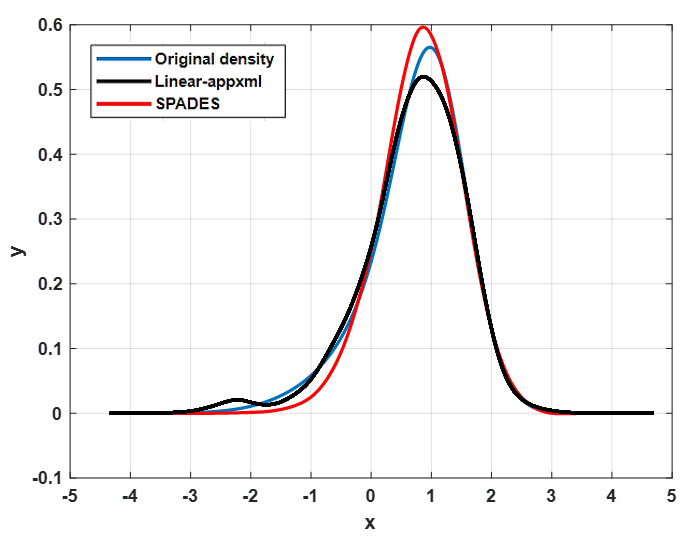
\includegraphics[scale = 0.36]{Figures/Adaptive/cmp_reults/2.PNG} \\
         \begin{tabular}{c}Averge $MSE_{Proposed} = 5.1808e-04$ \\ Average $MSE_{SPADES} =4.1e-03$\end{tabular}&\begin{tabular}{c}Averge $MSE_{Proposed} = 2.7e-03$\\ $Average MSE_{SPADES} =2.3e-02$\end{tabular}&\begin{tabular}{c}Averge $MSE_{Proposed} = 4.5e-03$ \\ Average $MSE_{SPADES} =2.2e-02$\end{tabular}\\
         $f_3$& $f_4$ & $f_5$\\
          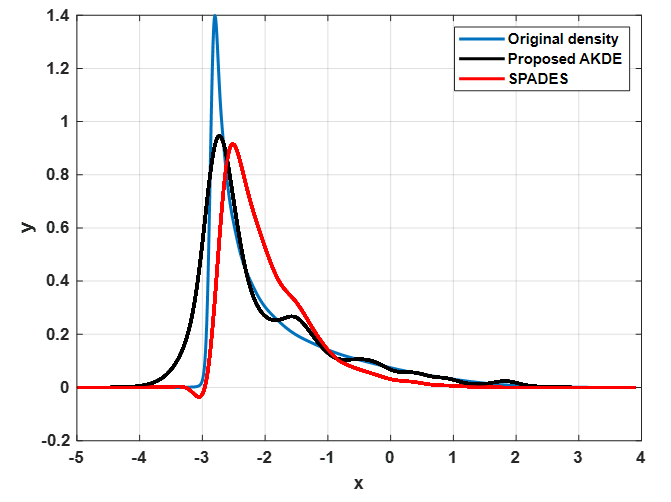
\includegraphics[scale = 0.38]{Figures/Adaptive/cmp_reults/3.PNG}&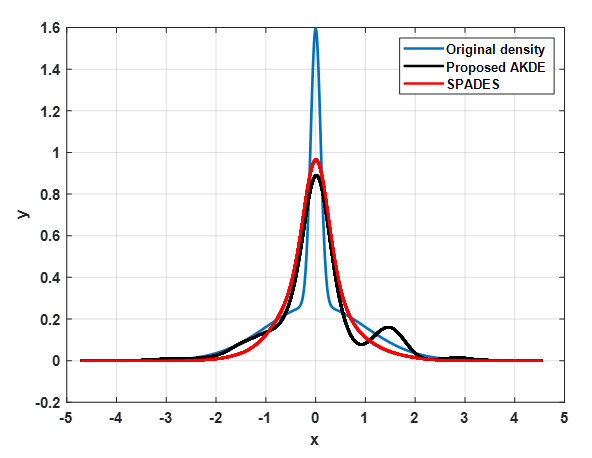
\includegraphics[scale = 0.43]{Figures/Adaptive/cmp_reults/4.PNG}&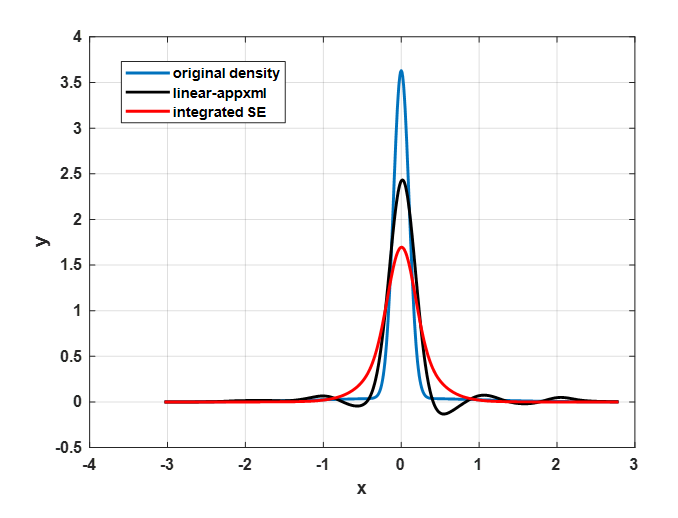
\includegraphics[scale = 0.4]{Figures/Adaptive/cmp_reults/5.PNG} \\
          \begin{tabular}{c}Averge $MSE_{Proposed} = 6.0e-02$ \\ Average $MSE_{SPADES} =3.4e-02$\end{tabular}&\begin{tabular}{c}Averge $MSE_{Proposed} = 1.6e-01$ \\ Average $MSE_{SPADES} =5.3e-02$\end{tabular}&\begin{tabular}{c}Averge $MSE_{Proposed} = 3.1$ \\ Average $MSE_{SPADES} =2.4e-01$\end{tabular}\\
          $f_6$& $f_7$ & $f_8$\\
           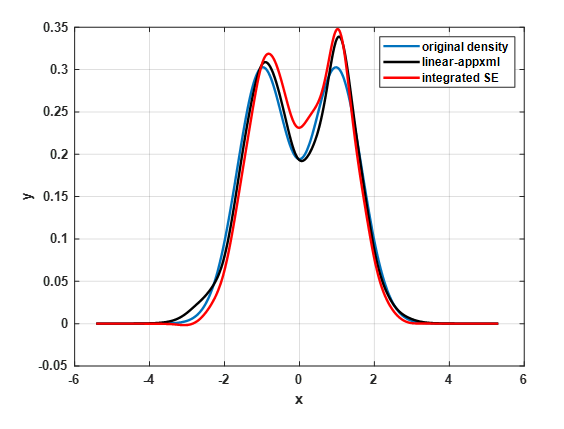
\includegraphics[scale = 0.45]{Figures/Adaptive/cmp_reults/6.PNG}&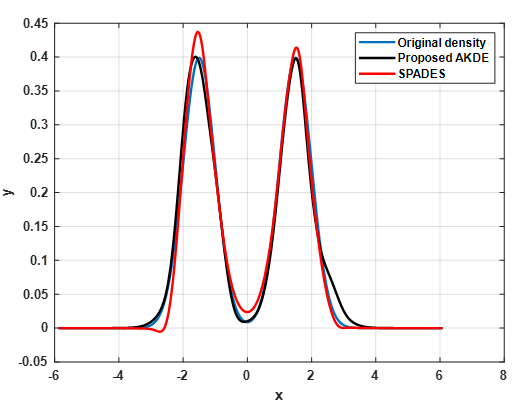
\includegraphics[scale = 0.45]{Figures/Adaptive/cmp_reults/7.PNG}&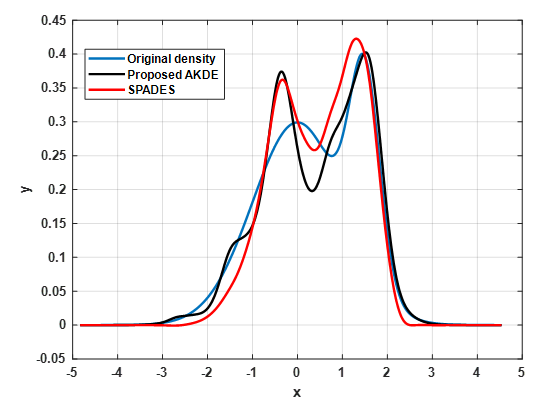
\includegraphics[scale = 0.45]{Figures/Adaptive/cmp_reults/8.PNG} \\
          \begin{tabular}{c}Averge $MSE_{Proposed} = 3.1e-03$ \\ Average $MSE_{SPADES} =1.9e-02$\end{tabular}&\begin{tabular}{c}Averge $MSE_{Proposed} = 3.0e-03$ \\ Average $MSE_{SPADES} =2.1e-02$\end{tabular}&\begin{tabular}{c}Averge $MSE_{Proposed} = 3.6e-03$ \\ Average $MSE_{SPADES} =1.8e-02$\end{tabular}\\
          $f_{9}$& $f_{10}$ & $f_{11}$\\
          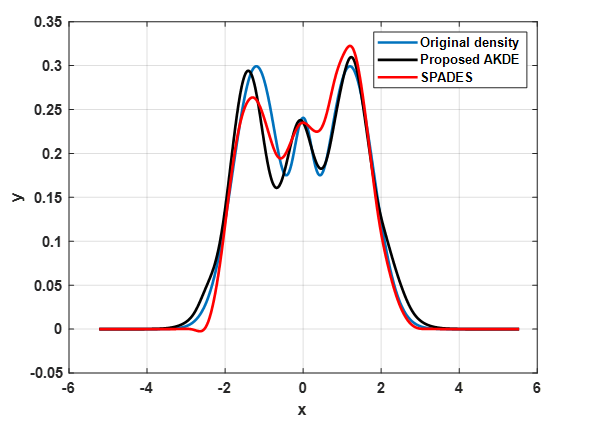
\includegraphics[scale = 0.46]{Figures/Adaptive/cmp_reults/9.PNG}&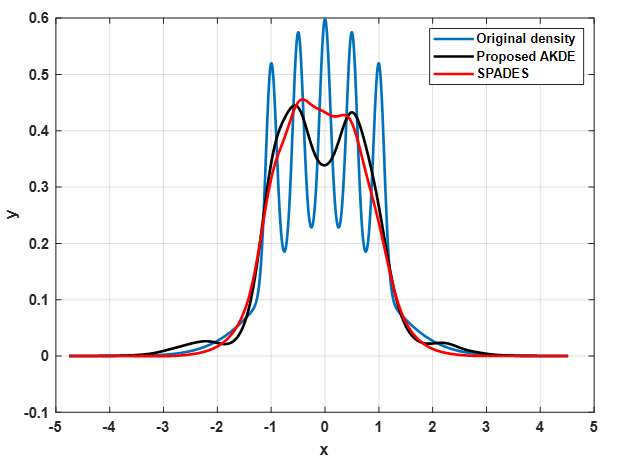
\includegraphics[scale = 0.45]{Figures/Adaptive/cmp_reults/10.PNG}&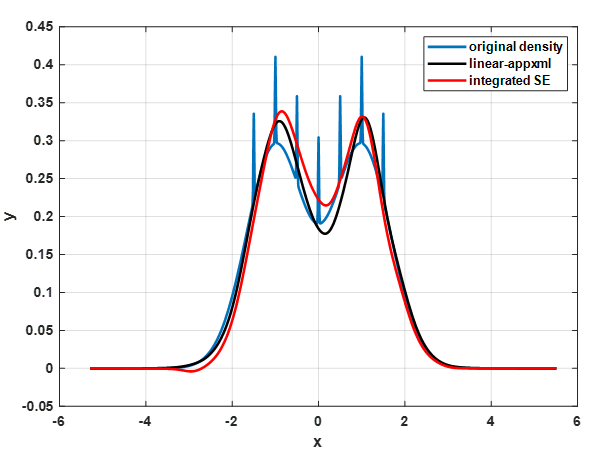
\includegraphics[scale = 0.45]{Figures/Adaptive/cmp_reults/11.PNG} \\
          \begin{tabular}{c}Averge $MSE_{Proposed} = 3.0e-03$ \\ Average $MSE_{SPADES} =1.3e-02$\end{tabular}&\begin{tabular}{c}Averge $MSE_{Proposed} = 2.0e-02$ \\ Average $MSE_{SPADES} =1.6e-02$\end{tabular}&\begin{tabular}{c}Averge $MSE_{Proposed} = 2.6e-03$ \\ Average $MSE_{SPADES} =1.2e-02$\end{tabular}\\
          $f_{12}$& $f_{13}$ & $f_{14}$\\
          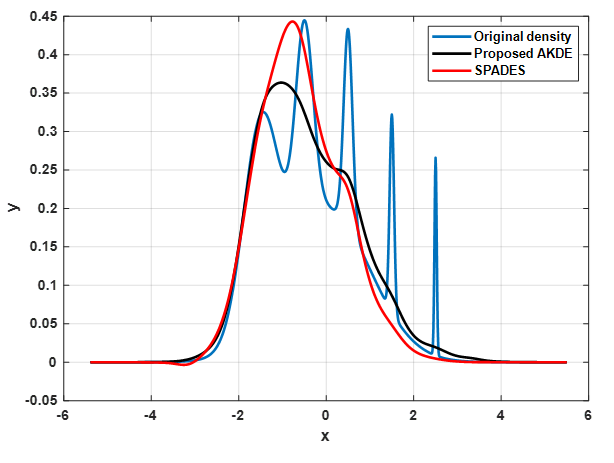
\includegraphics[scale = 0.46]{Figures/Adaptive/cmp_reults/12.PNG}&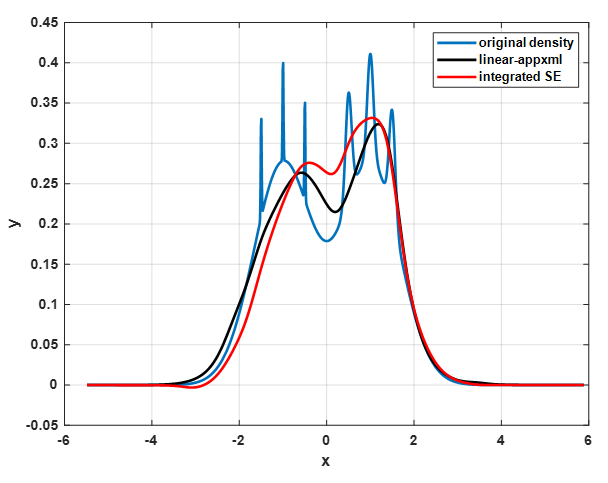
\includegraphics[scale = 0.45]{Figures/Adaptive/cmp_reults/13.PNG}&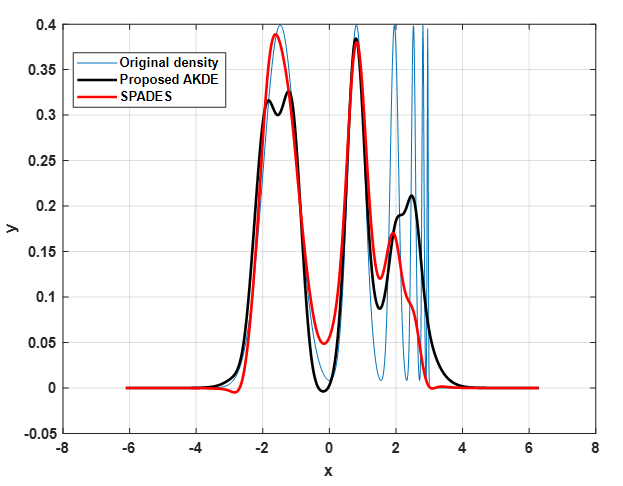
\includegraphics[scale = 0.45]{Figures/Adaptive/cmp_reults/14.PNG} \\
          \begin{tabular}{c}Averge $MSE_{Proposed} = 8.4e-03$ \\ Average $MSE_{SPADES} =1.6e-02$\end{tabular}&\begin{tabular}{c}Averge $MSE_{Proposed} = 4.1e-03$ \\ Average $MSE_{SPADES} =1.5e-02$\end{tabular}&\begin{tabular}{c}Averge $MSE_{Proposed} = 2.4e-02$ \\ Average $MSE_{SPADES} =2.0e-02$\end{tabular}\\
    \end{tabular}
    \caption{Results obtained by proposed method (marked as black) compared to  SPADES~\cite{bunea2010spades} (marked as red) method for nonparametric adaptive kernel density estimation.}
    \label{fig:cmp_res}
\end{figure}
%%%%%%%%%%%%%%%%%%%%%%%%%%%%%%%%%%%%%%%%%%%%%%%
Figure~\ref{fig:N} shows average MSE over 10 runs for proposed AKDE and spades methods. We set $pq = 600, \gamma = 7$ for this experiment.
\begin{figure}
    \hspace{-1cm}
    \begin{tabular}{ccc}
    $f_{0}$& $f_{1}$ & $f_{2}$\\
        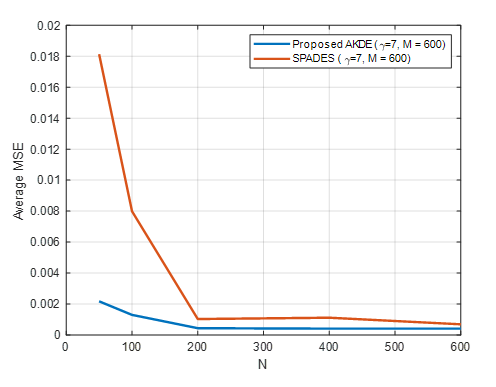
\includegraphics[scale = 0.5]{Figures/Adaptive/N/0.PNG} & 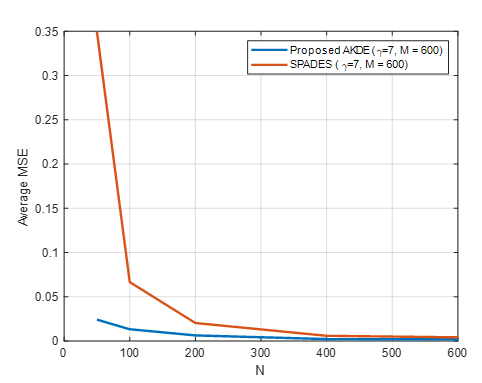
\includegraphics[scale = 0.5]{Figures/Adaptive/N/1.PNG} & 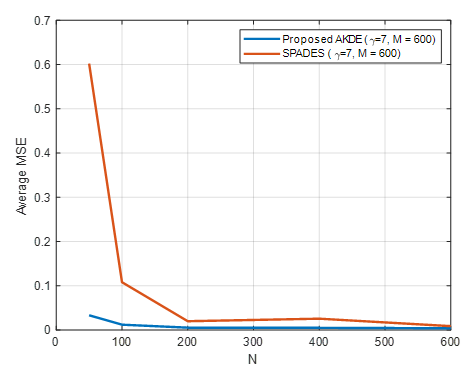
\includegraphics[scale = 0.5]{Figures/Adaptive/N/2.PNG}   \\
    $f_{3}$& $f_{4}$ & $f_{5}$\\
        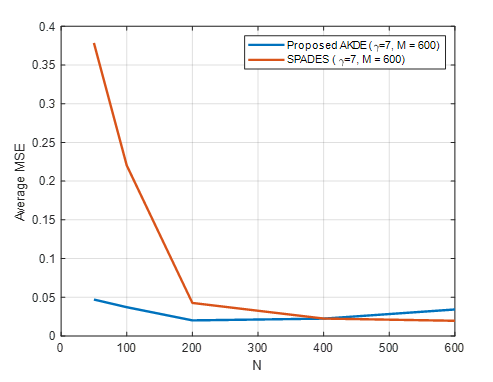
\includegraphics[scale = 0.5]{Figures/Adaptive/N/3.PNG} & 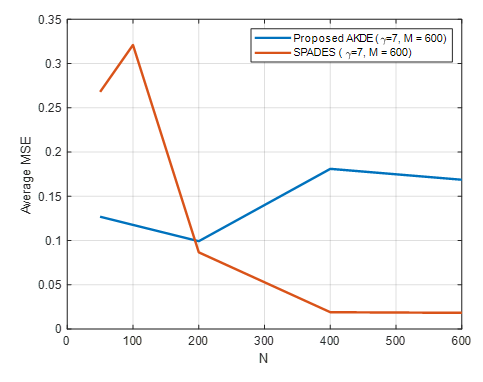
\includegraphics[scale = 0.5]{Figures/Adaptive/N/4.PNG} & 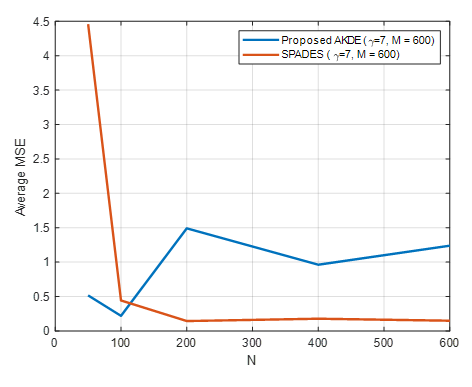
\includegraphics[scale = 0.5]{Figures/Adaptive/N/5.PNG}   \\
    $f_{6}$& $f_{7}$ & $f_{8}$\\
        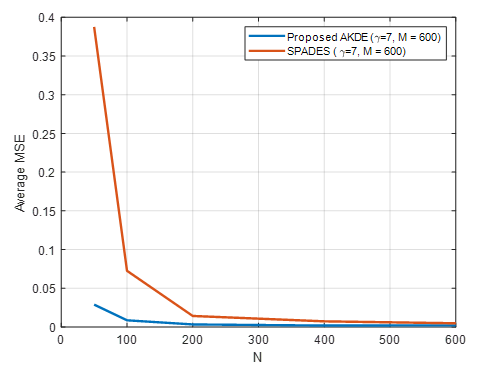
\includegraphics[scale = 0.5]{Figures/Adaptive/N/6.PNG} & 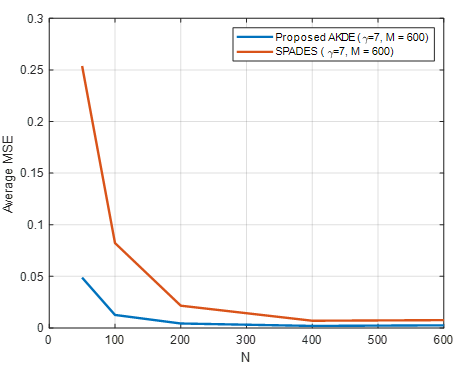
\includegraphics[scale = 0.5]{Figures/Adaptive/N/7.PNG} & 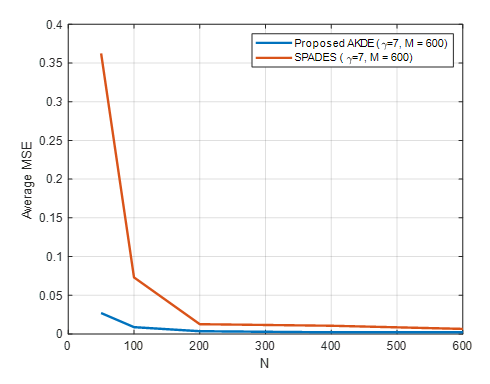
\includegraphics[scale = 0.5]{Figures/Adaptive/N/8.PNG}   \\
    $f_{9}$& $f_{10}$ & $f_{11}$\\
        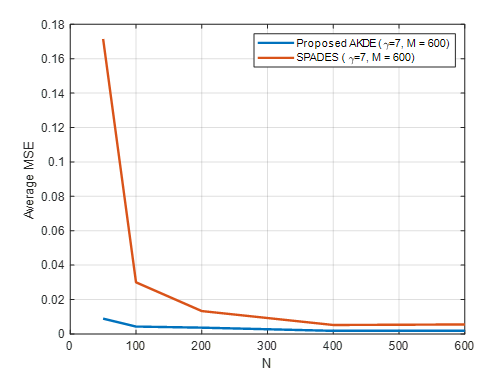
\includegraphics[scale = 0.5]{Figures/Adaptive/N/9.PNG} & 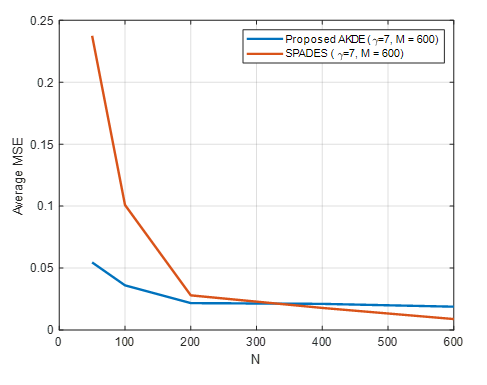
\includegraphics[scale = 0.5]{Figures/Adaptive/N/10.PNG} & 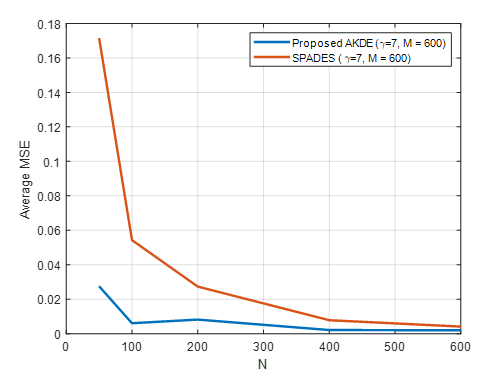
\includegraphics[scale = 0.5]{Figures/Adaptive/N/11.PNG}   \\
    $f_{12}$& $f_{13}$ & $f_{14}$\\
        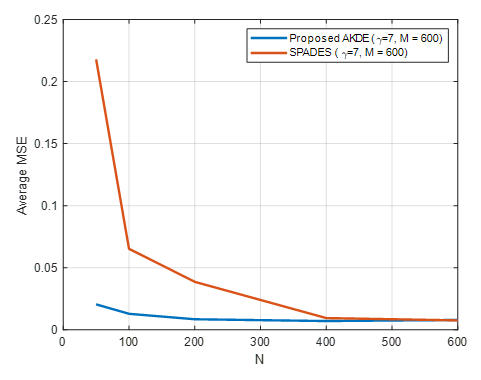
\includegraphics[scale = 0.5]{Figures/Adaptive/N/12.PNG} & 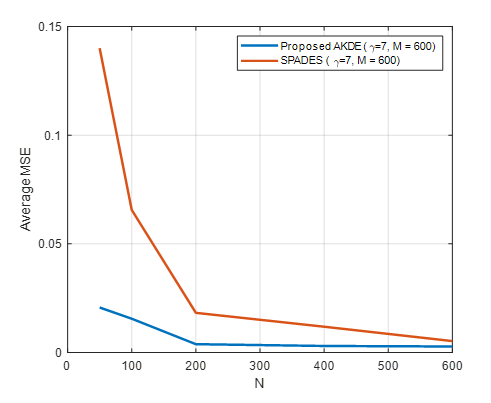
\includegraphics[scale = 0.5]{Figures/Adaptive/N/13.PNG} & 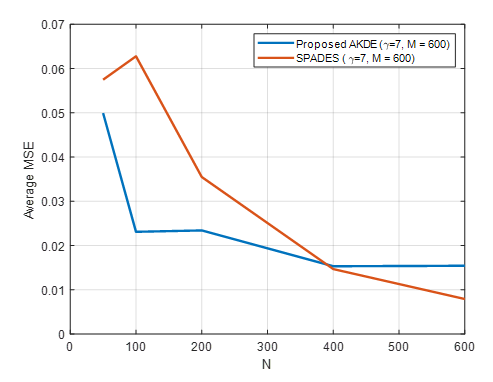
\includegraphics[scale = 0.5]{Figures/Adaptive/N/14.PNG}   \\
         
    \end{tabular}
    
    \caption{Diagram of MSE v.s. number of samples drawn from each density for 15 one dimensional densities.}
    \label{fig:N}
\end{figure}